\section{Sample Motion Law Processing Output}%
\label{sec:sample_motion_law_processing_output}

	The current section shows and discusses sample output of the algorithm
	described in Section~\ref{sec:motion_law_generation_algorithm}. The current
	discussion relates to the planning problem and trajectory of
	Figure~\ref{fig:motion_law_sample_problem}.

	\begin{figure}[hb]
		\begin{minipage}{0.5\textwidth}
			\centering
			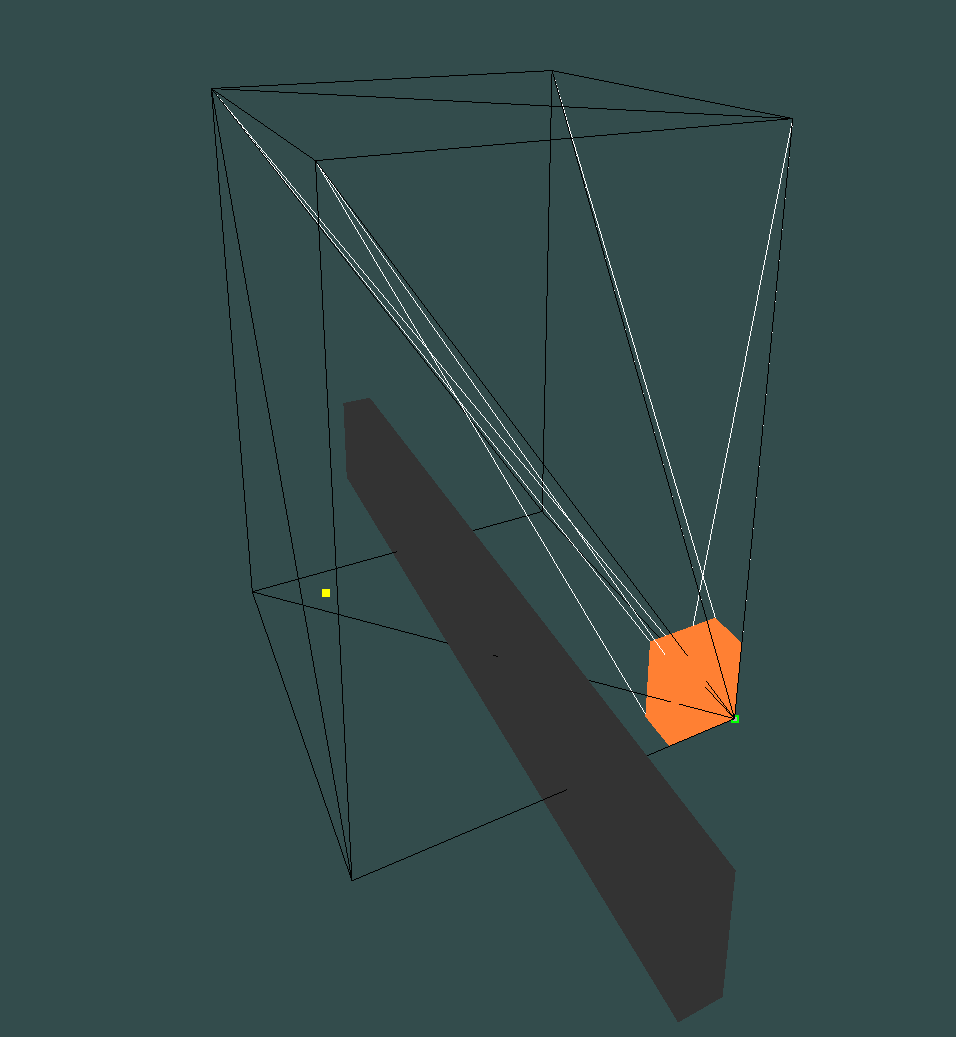
\includegraphics[height=0.6\textwidth]{kinematic_scaling_base_problem}
		\end{minipage}
		\begin{minipage}{0.5\textwidth}
			\centering
			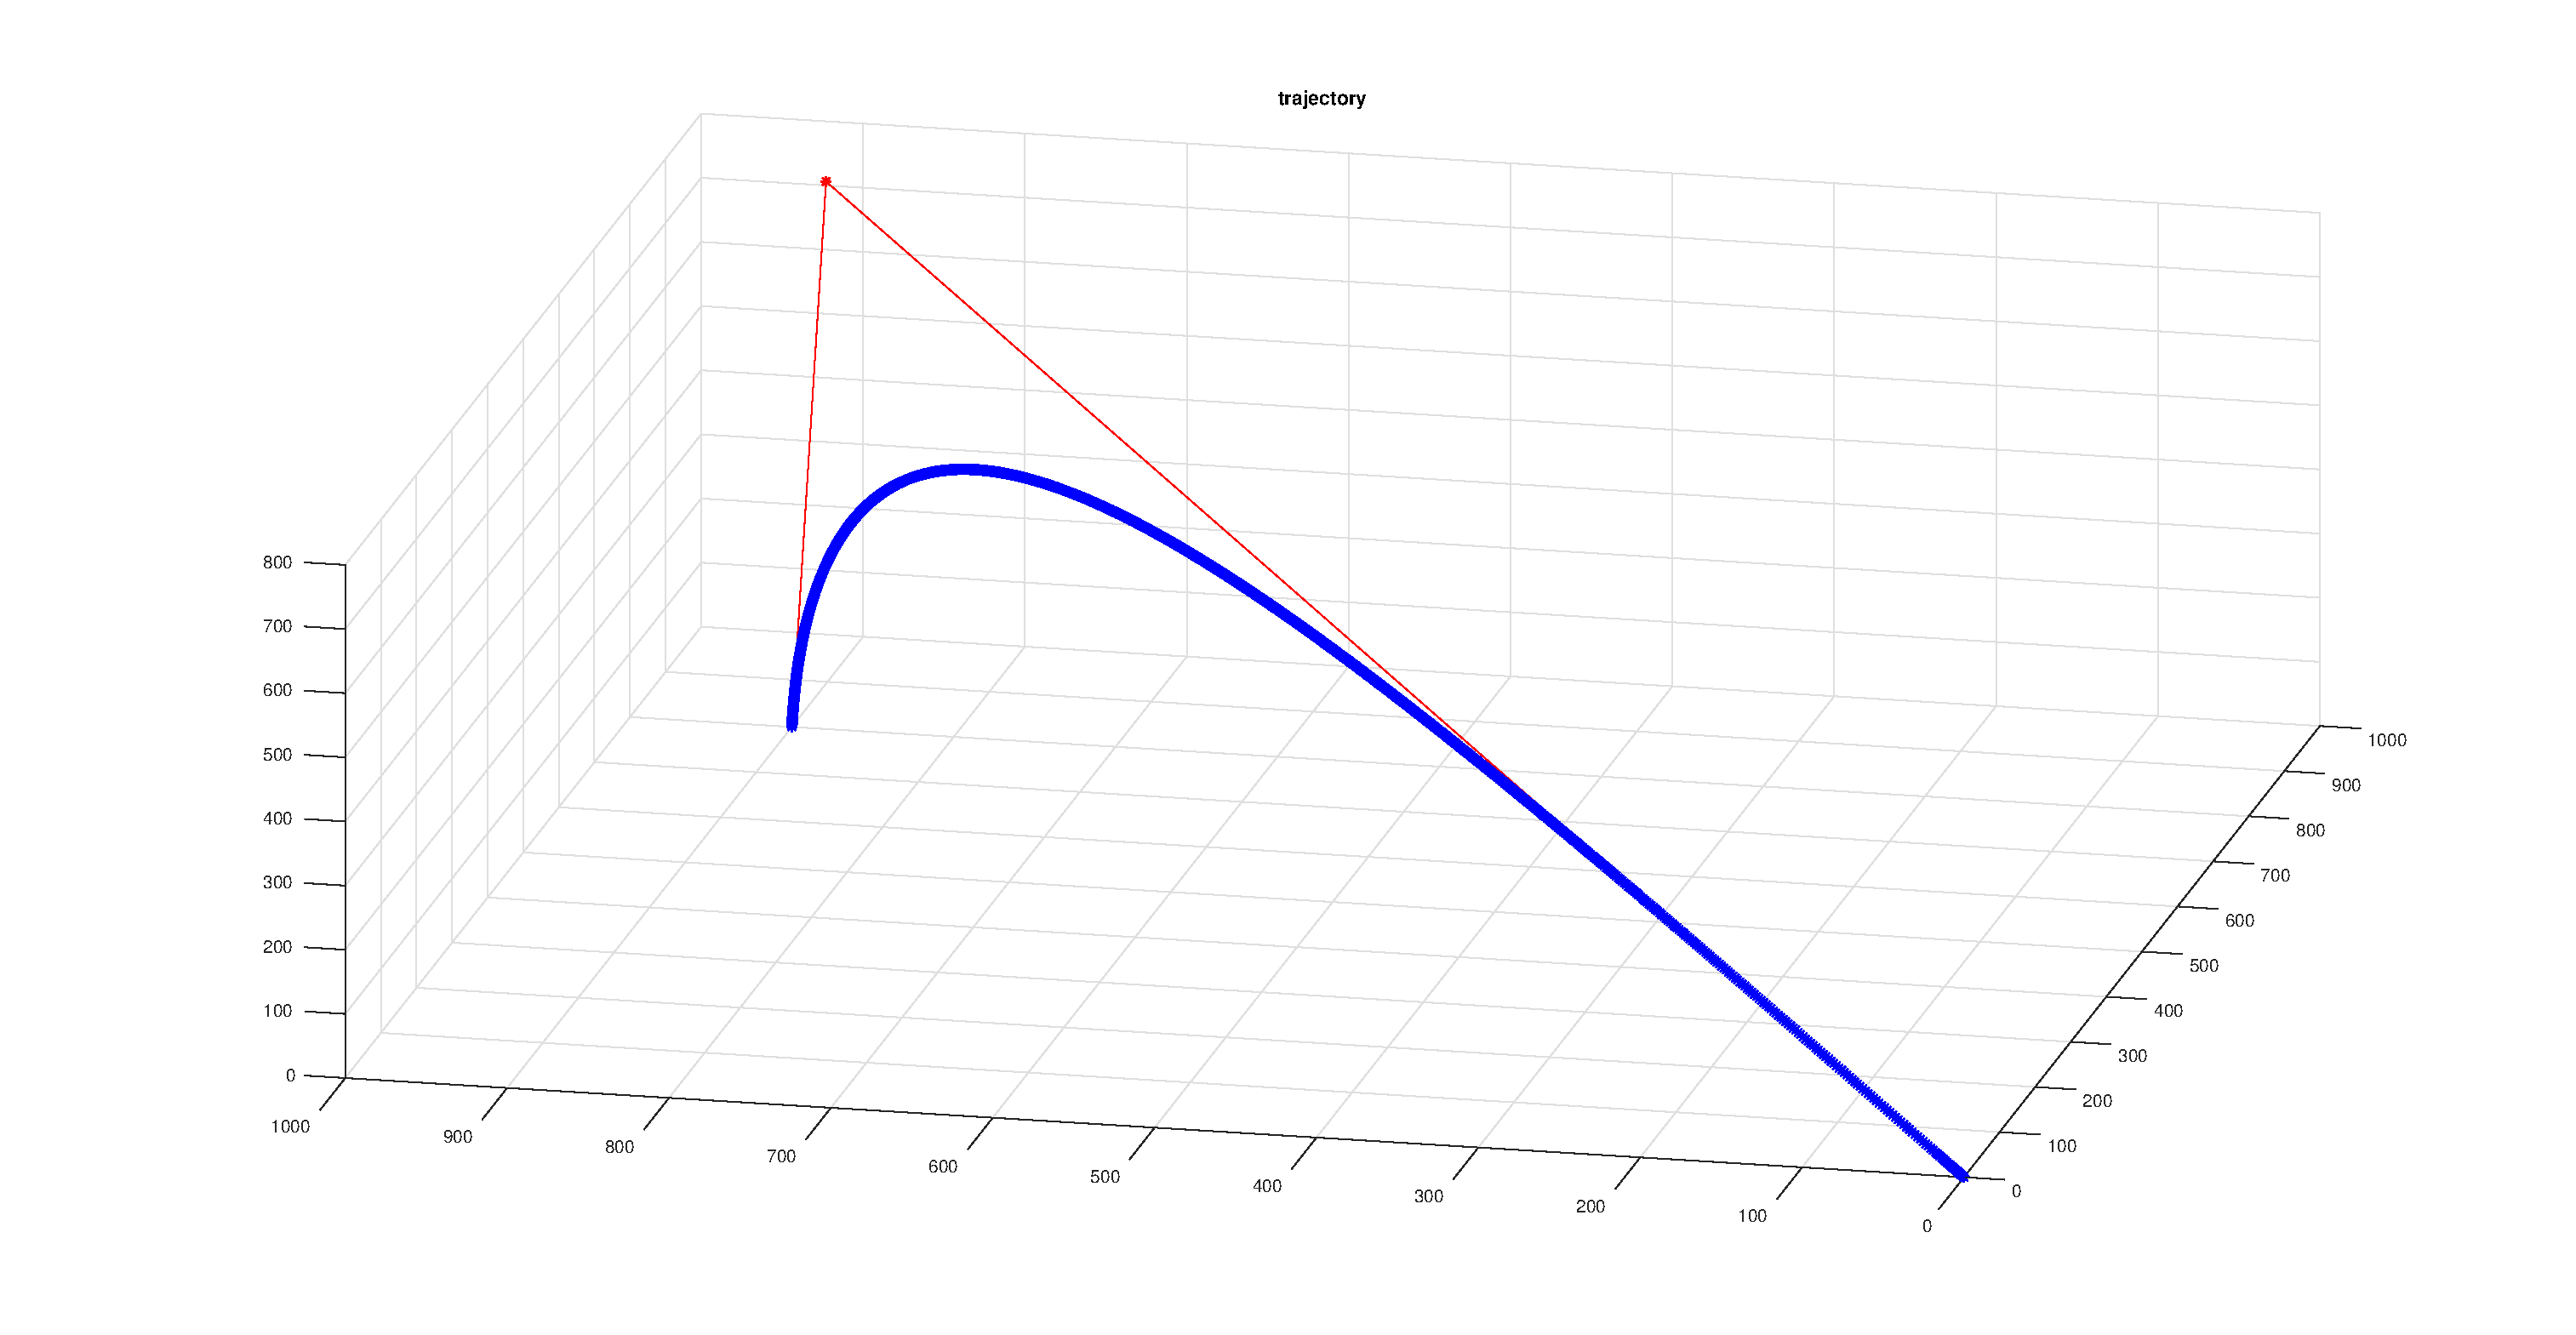
\includegraphics[height=0.6\textwidth]{motion_law_sample_problem_traj}
		\end{minipage}
		\caption[Motion Law Sample Problem]{Motion Law Sample Problem,
		left: problem layout, right: trajectory found}
		\label{fig:motion_law_sample_problem}
	\end{figure}

%	\begin{figure}[hbt!]
%		\begin{minipage}{0.5\textwidth}
%			\centering
%			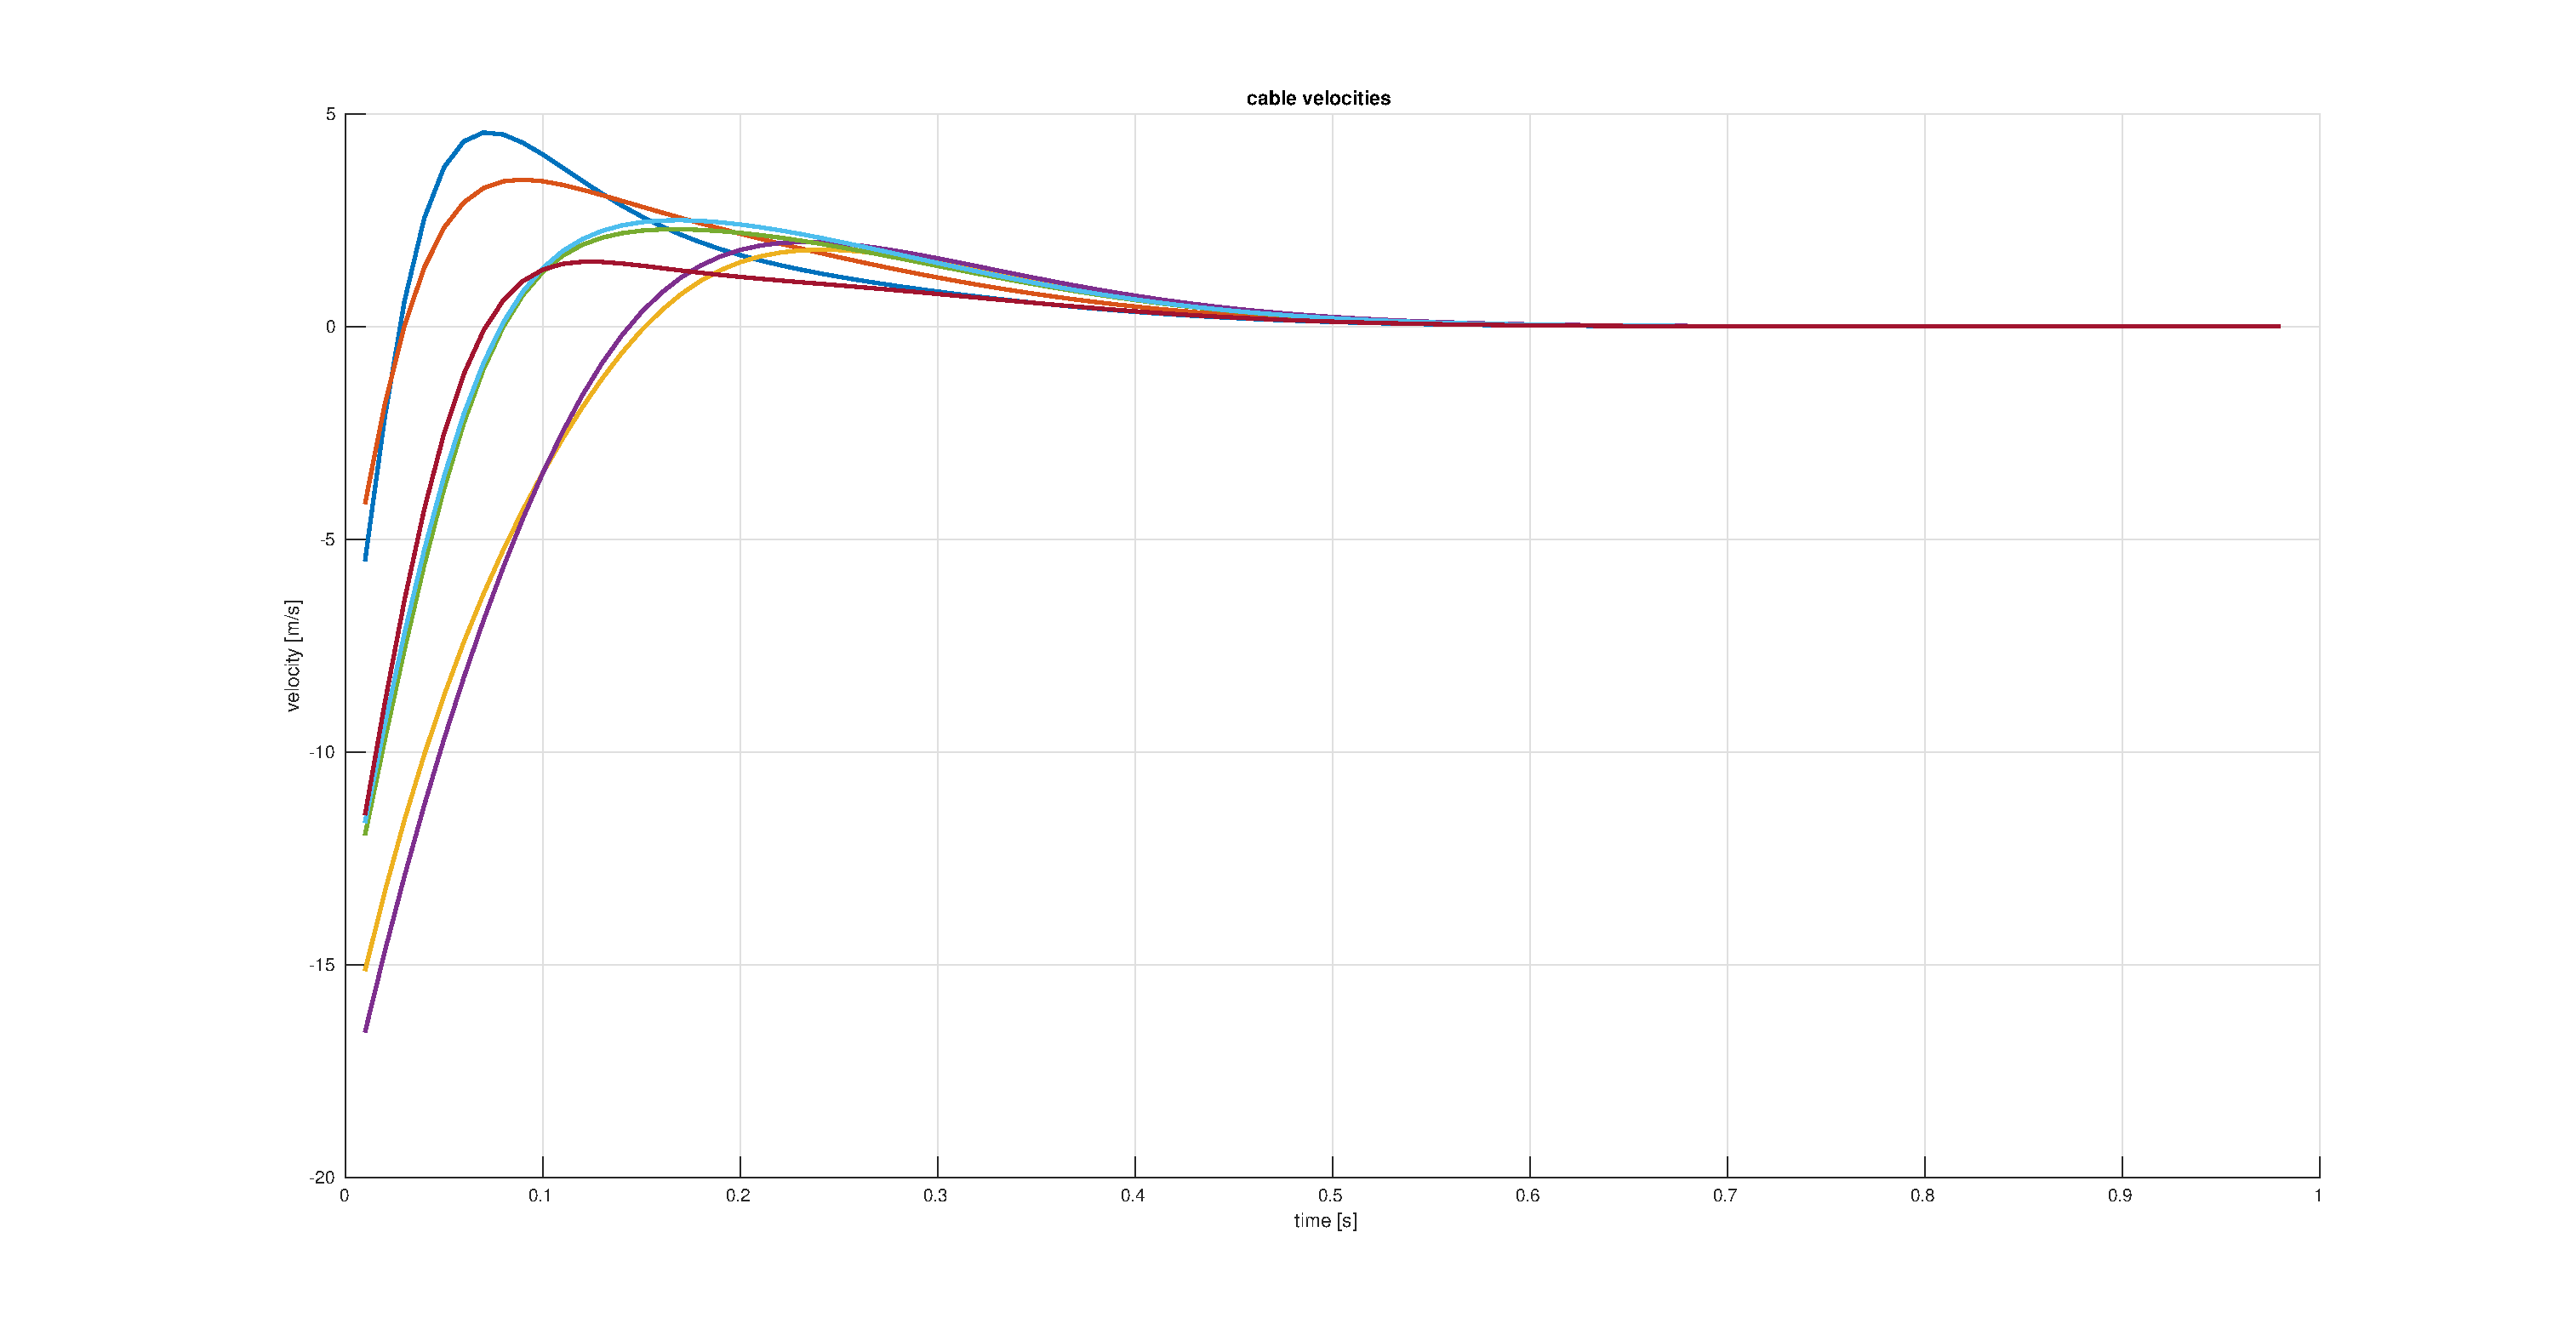
\includegraphics[width=\textwidth]{motion_law_base_velocities}
%			\caption{Cable Velocities without Motion Law Scaling}
%			\label{fig:cable_velocities_without_motion_law_scaling}
%		\end{minipage}
%		\begin{minipage}{0.5\textwidth}
%			\centering
%			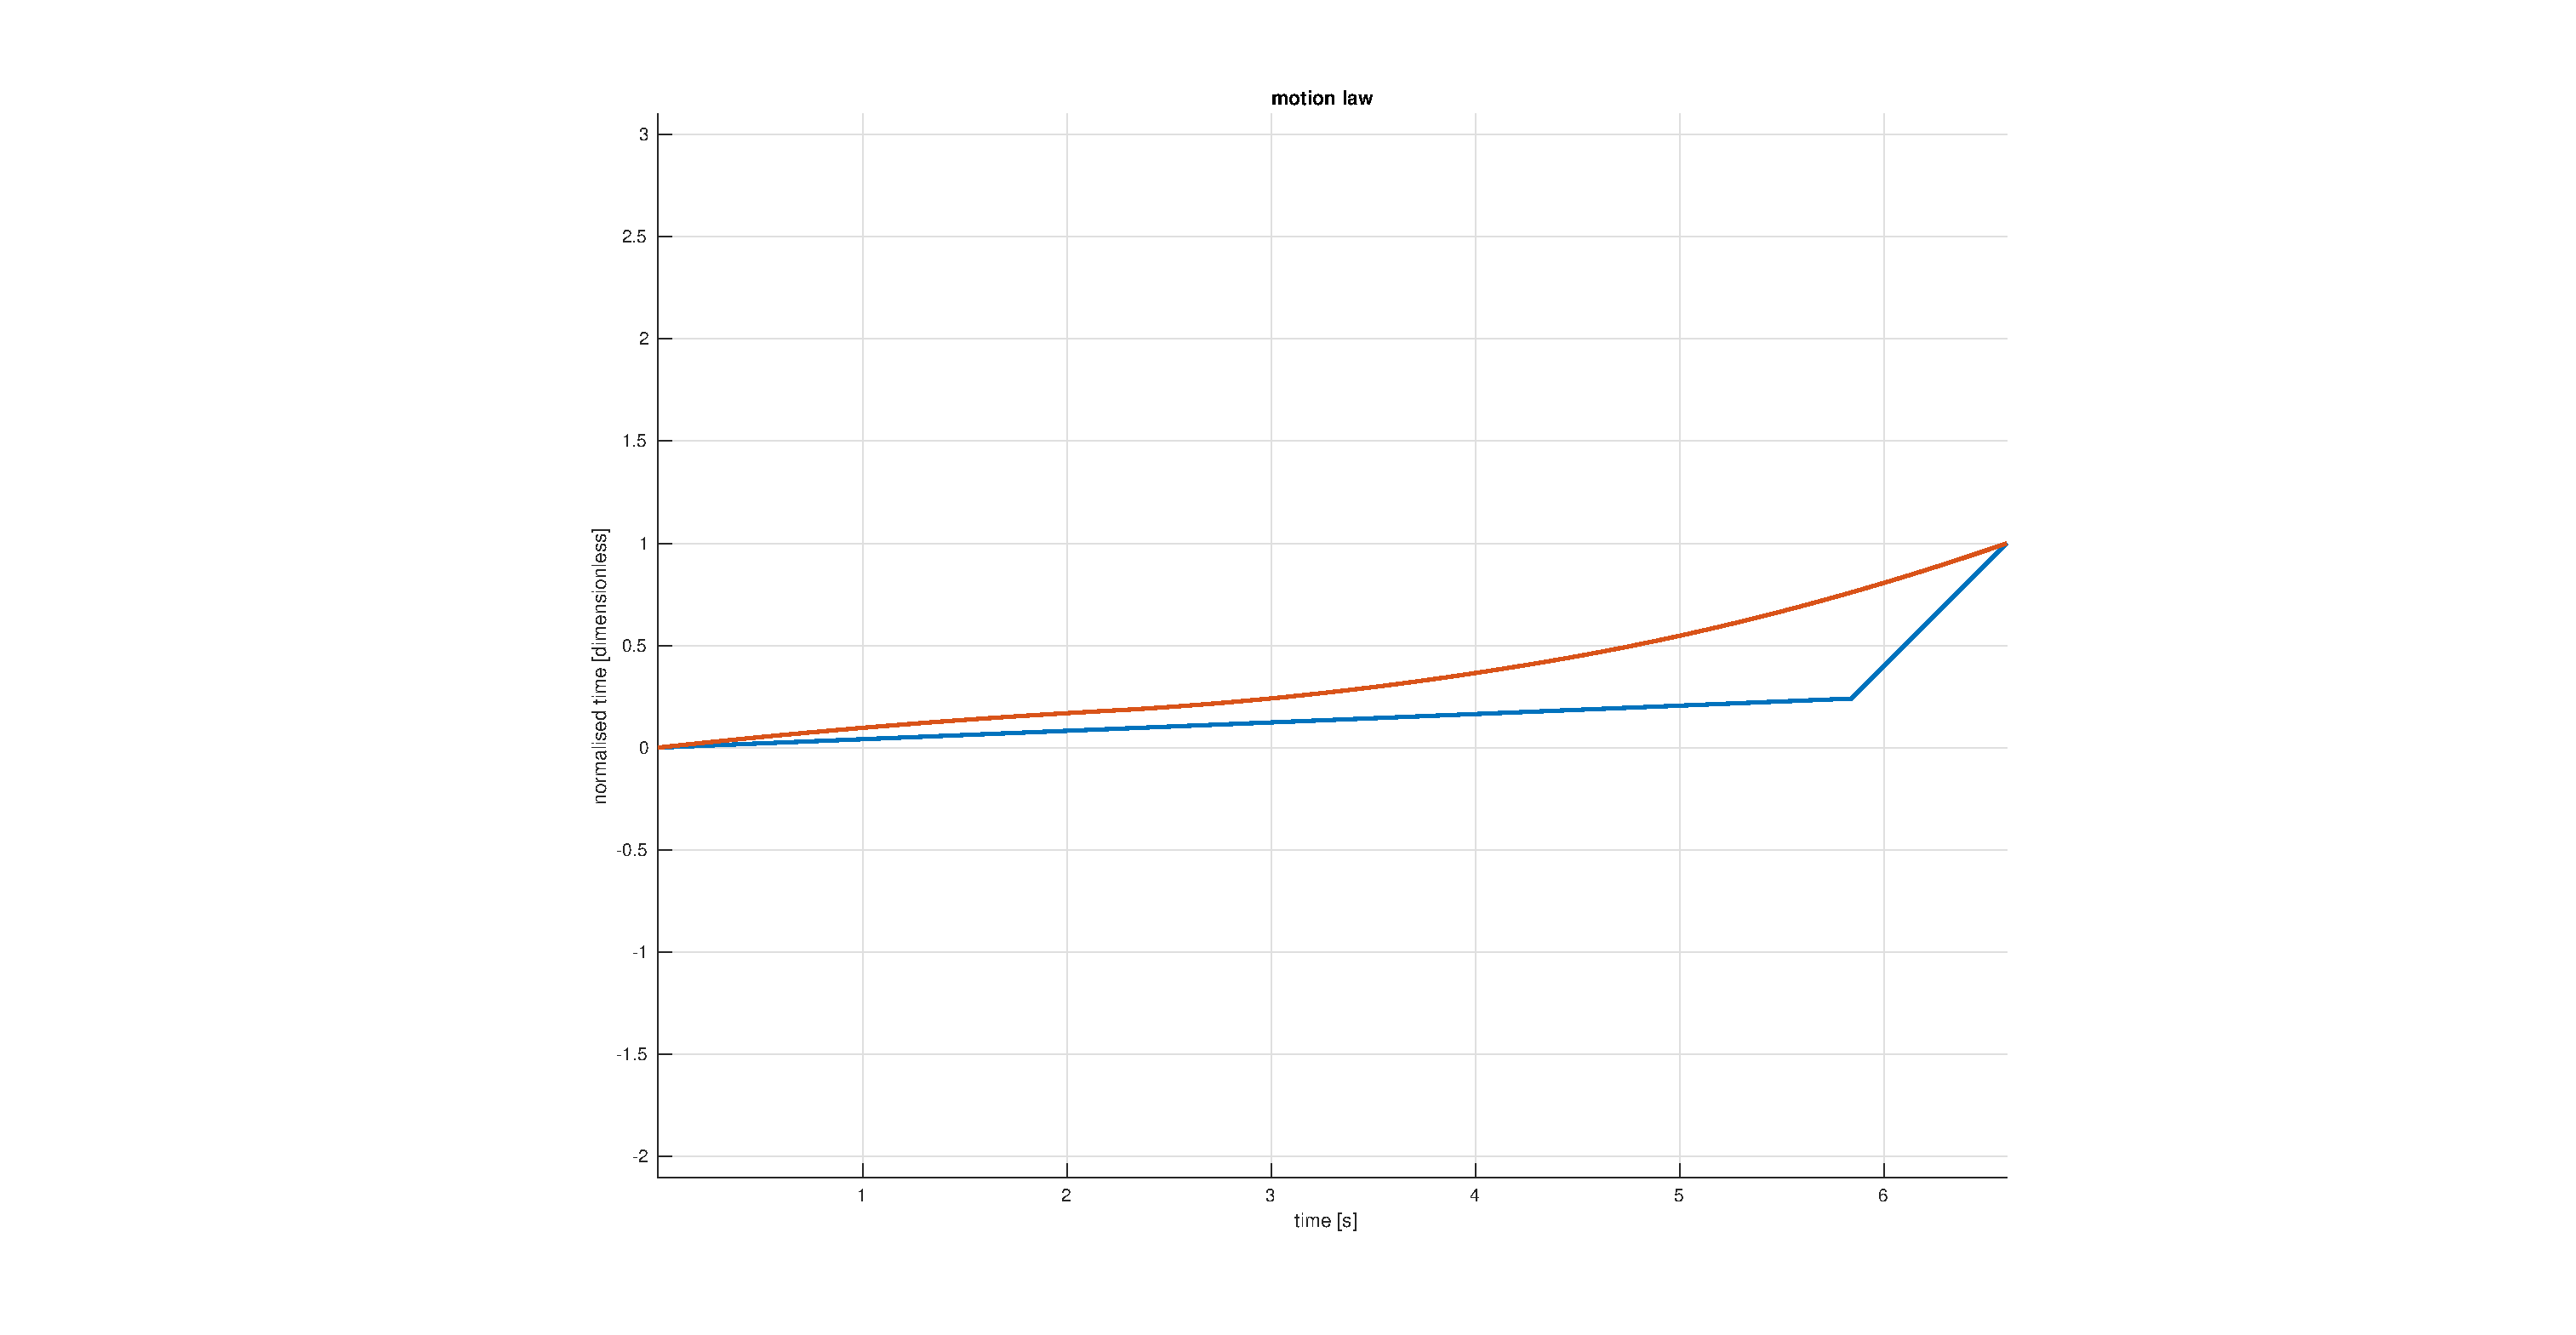
\includegraphics[width=\textwidth]{motion_law}
%			\caption{Cable Velocities with Motion Law Scaling}
%			\label{fig:motion_law}
%		\end{minipage}
%	\end{figure}
%
%	\begin{figure}[hbt!]
%		\begin{minipage}{0.5\textwidth}
%			\centering
%			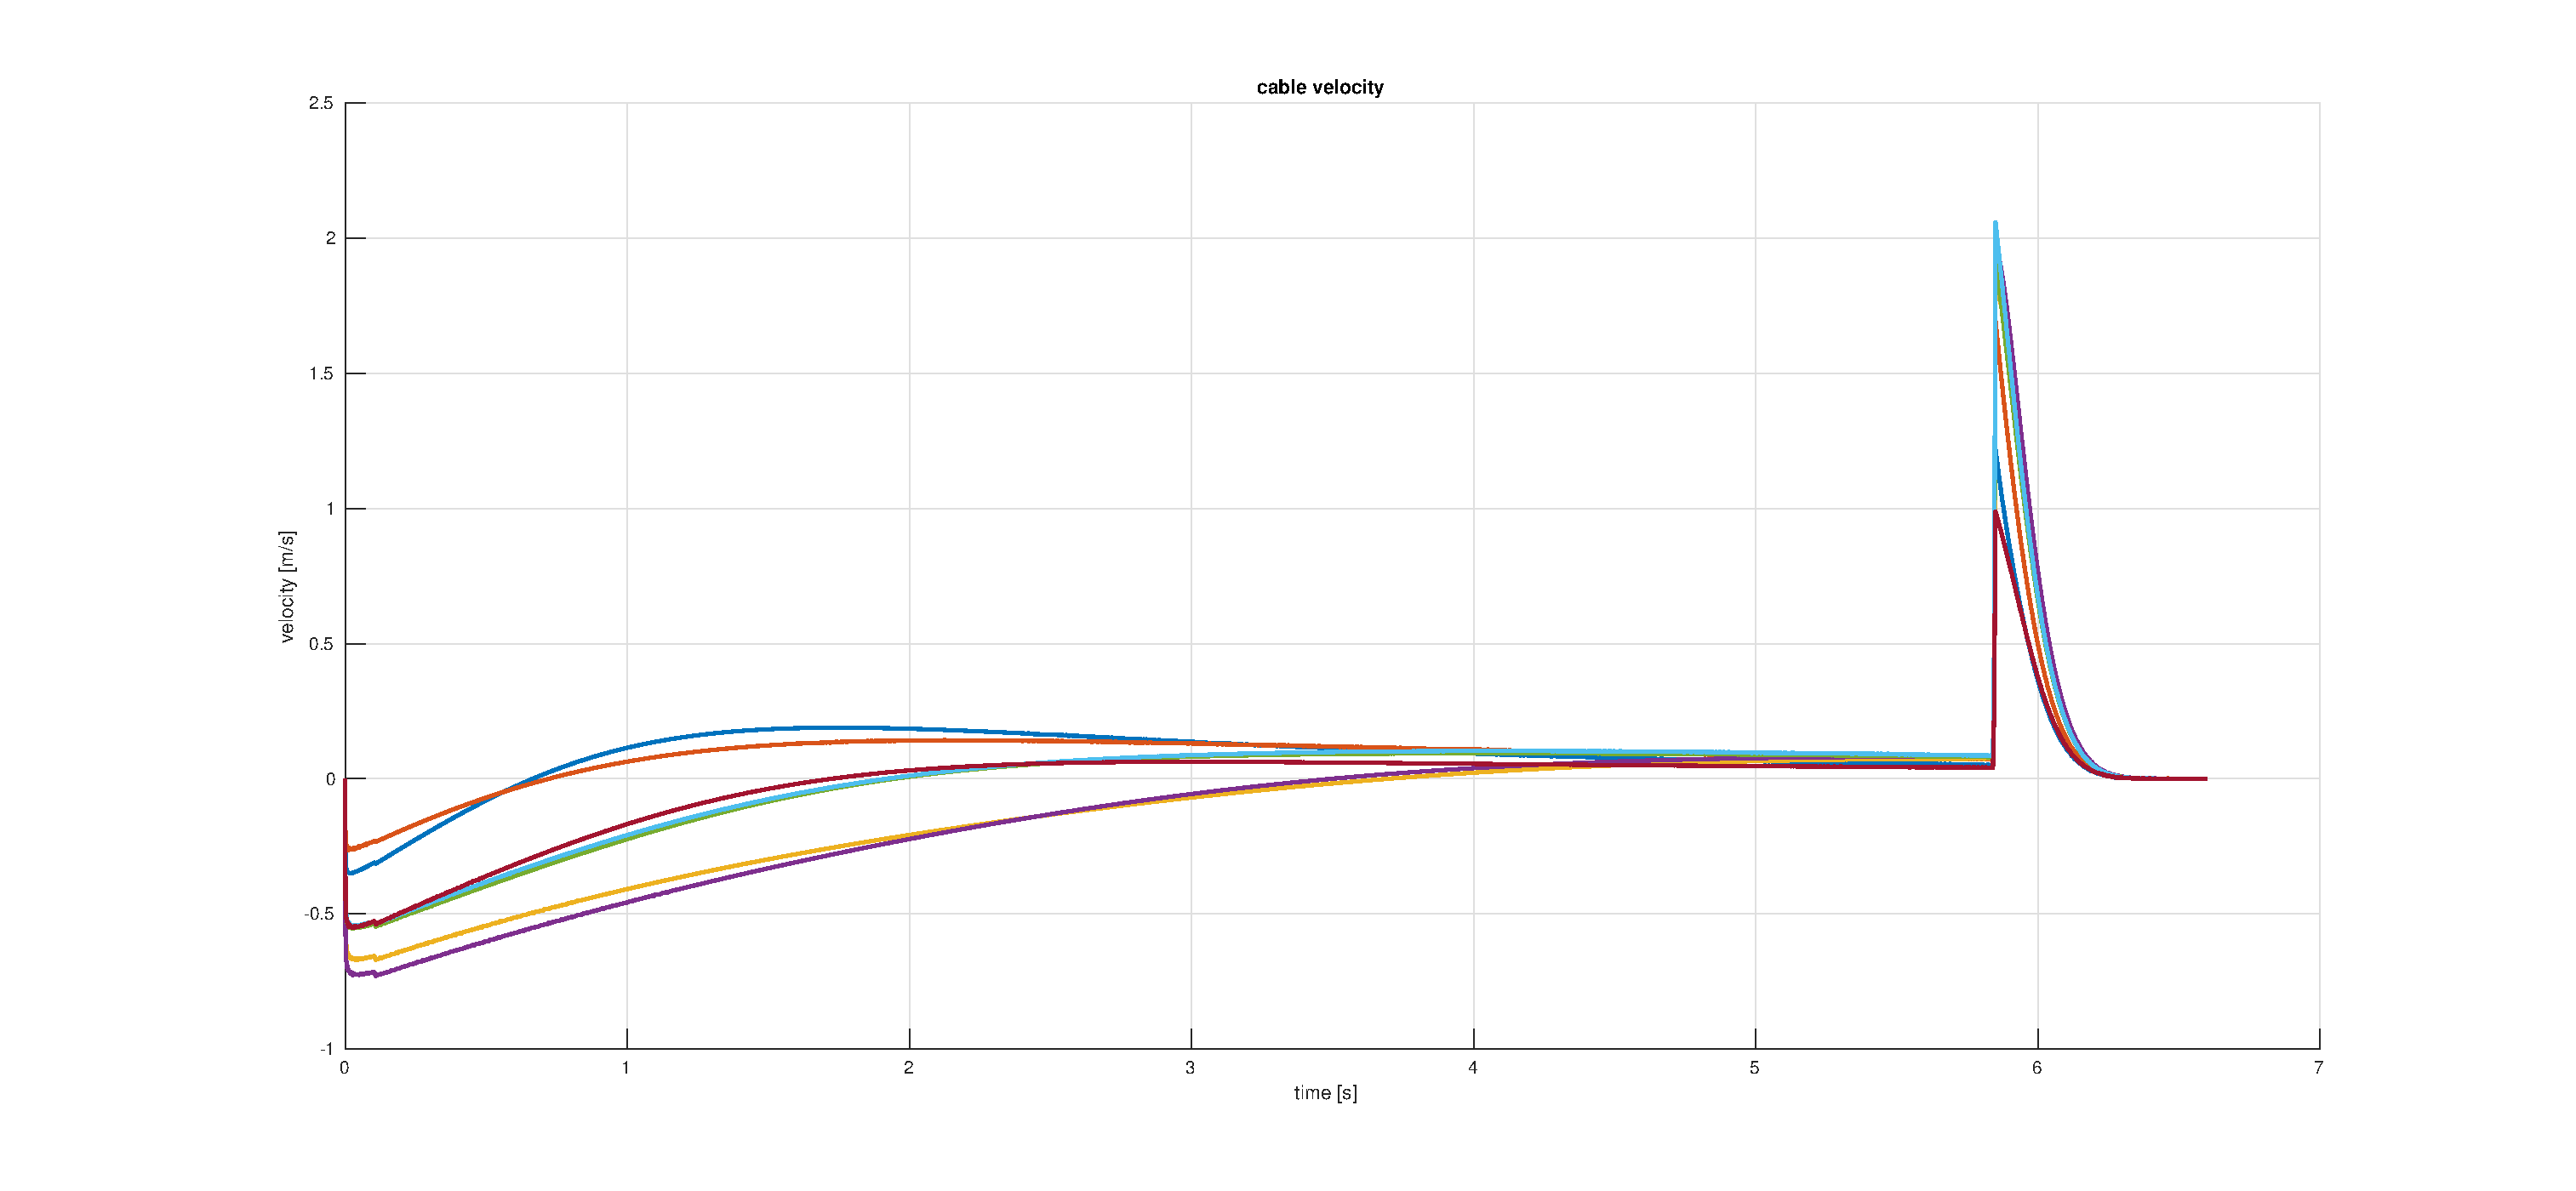
\includegraphics[width=\textwidth]{motion_law_output_velocities_no_spline}
%			\caption{Cable Velocities with Piecewise Linear Motion Law Scaling}
%			\label{fig:cable_velocities_with_motion_law_scaling_no_spline}
%		\end{minipage}
%		\begin{minipage}{0.5\textwidth}
%			\centering
%			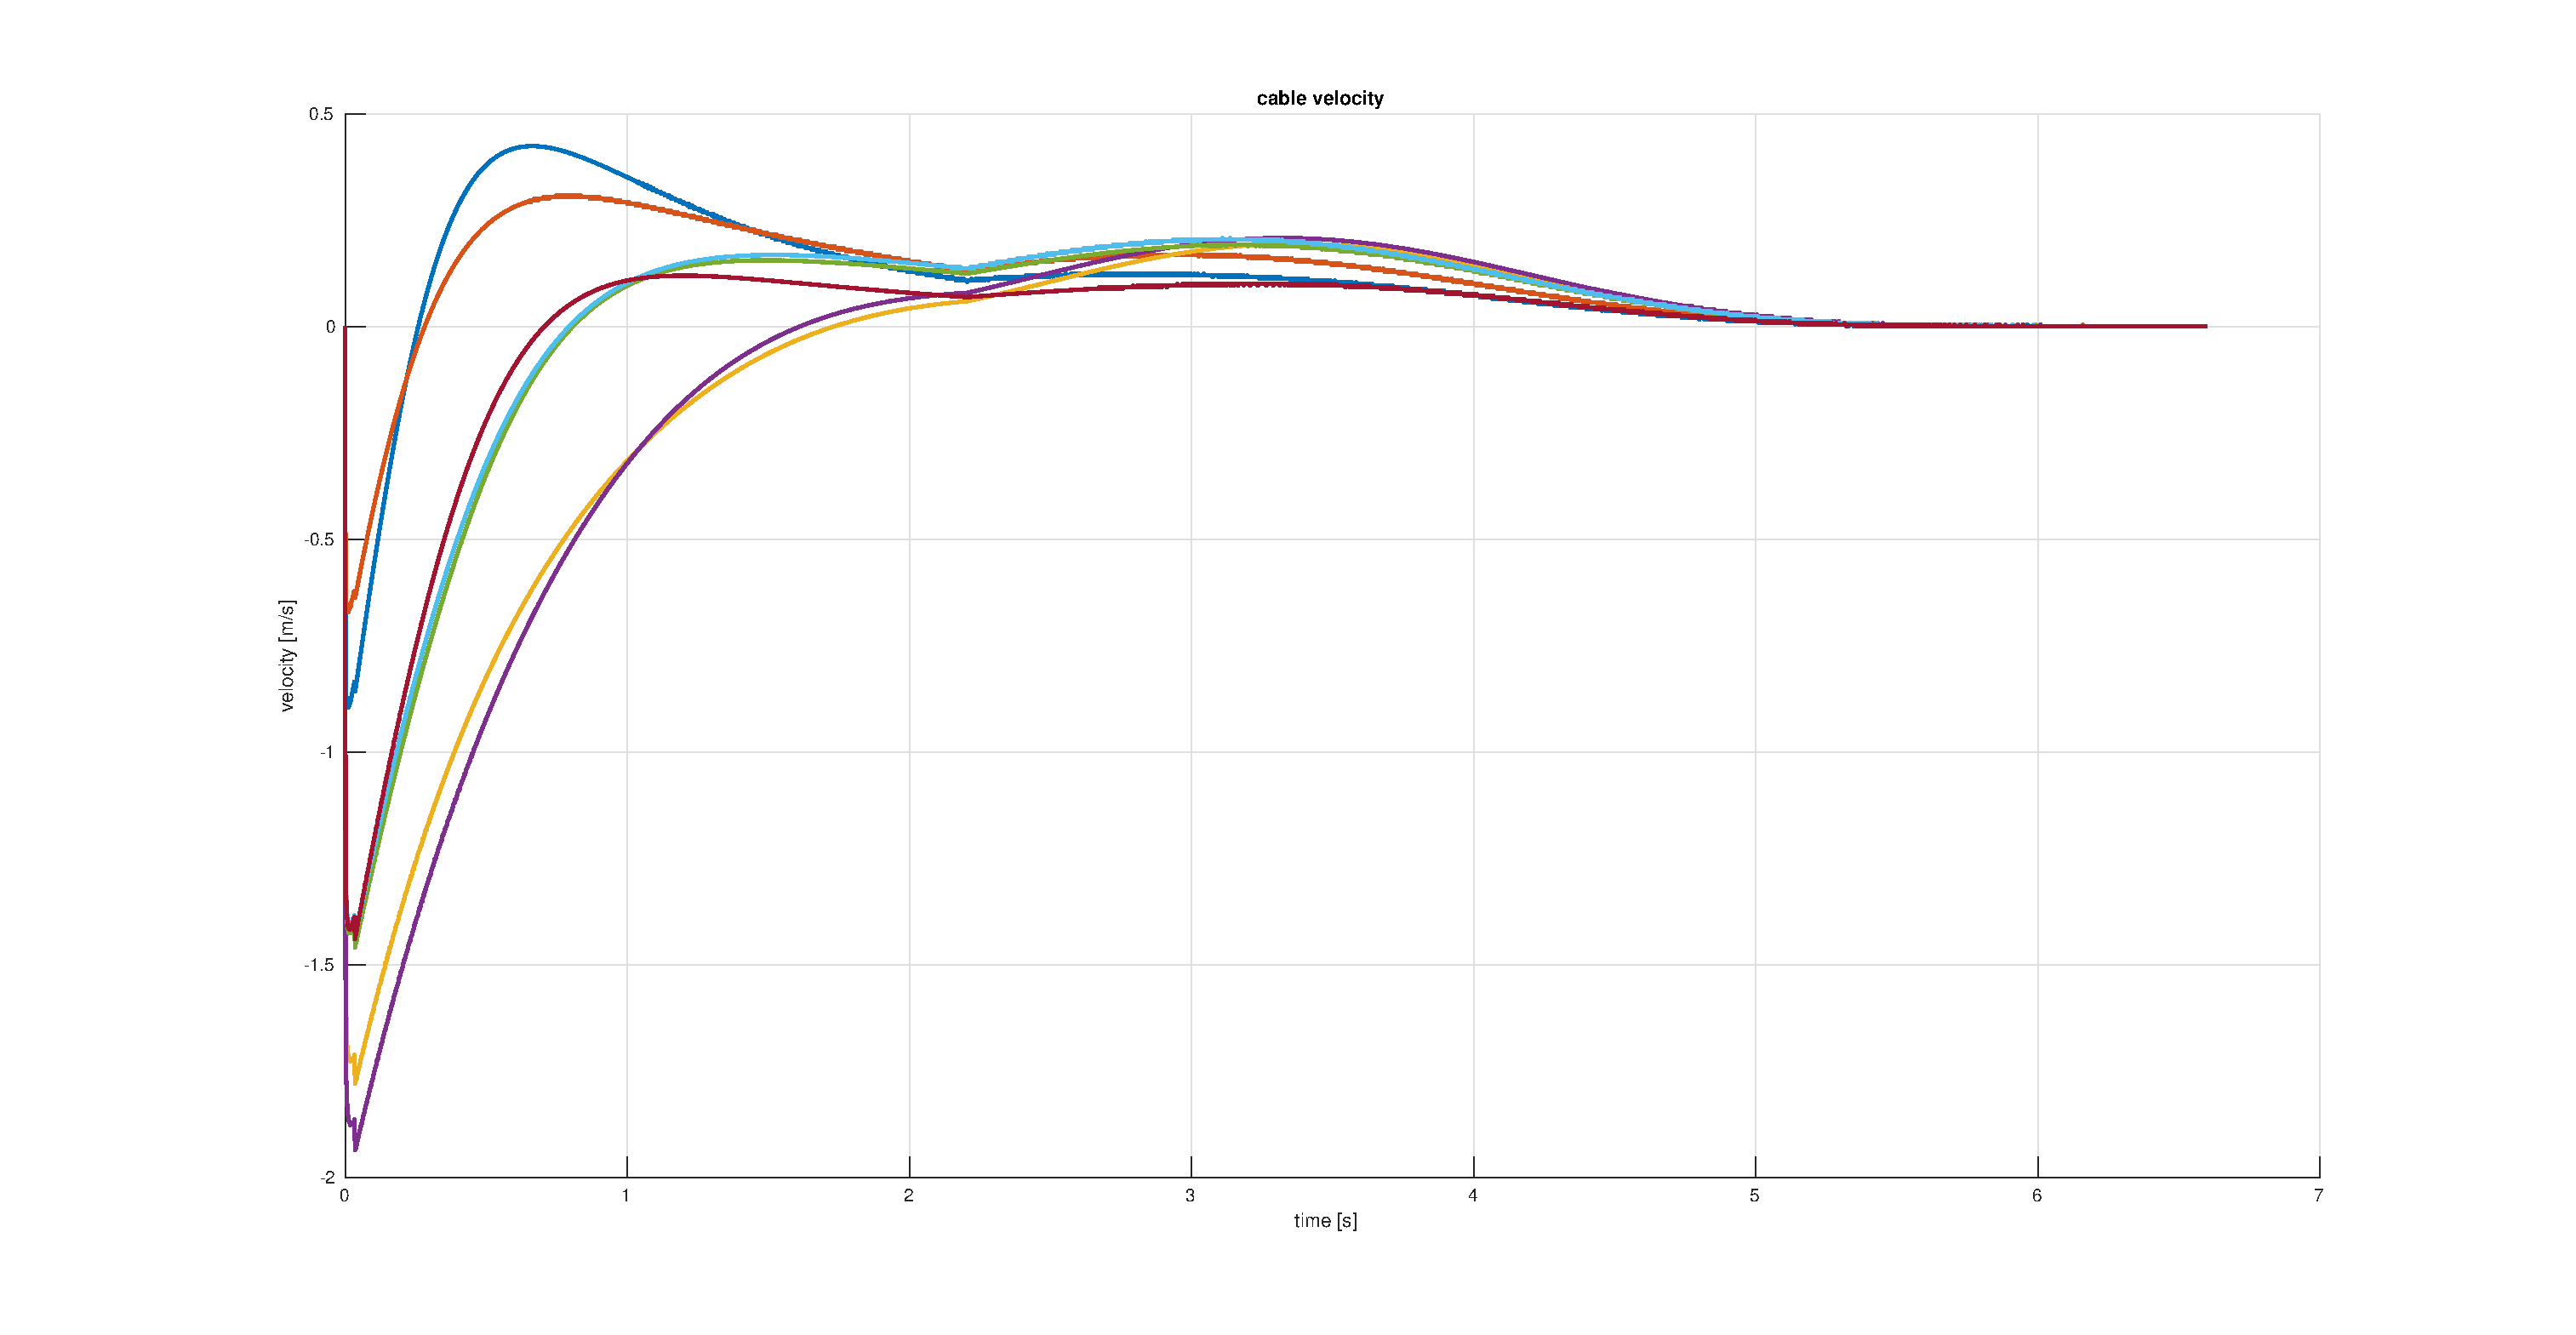
\includegraphics[width=\textwidth]{motion_law_output_velocities}
%			\caption{Cable Velocities with Motion Law Scaling}
%			\label{fig:cable_velocities_with_motion_law_scaling}
%		\end{minipage}
%	\end{figure}
%
%	The output of the algorithm for this problem is shown in
%	Figures
%	~\ref{fig:cable_velocities_without_motion_law_scaling},
%	~\ref{fig:motion_law},
%	~\ref{fig:cable_velocities_with_motion_law_scaling_no_spline},
%	and
%	~\ref{fig:cable_velocities_with_motion_law_scaling}.
%	In these figures, the algorithm attempted to find a motion law such that the
%	maximum velocity does not exceed $2\si{\meter\per\second}$. For comparison,
%	Figure~\ref{fig:cable_velocities_without_motion_law_scaling} shows the case
%	where the algorithm is not applied ($\timesym \defeq \timenorm$). As can be
%	seen, cable velocities reached up to $15\si{\meter\per\second}$ in this
%	case. The motion law generated by the algorithm is reported in
%	Figure~\ref{fig:motion_law}. In this figure both the control polygon and the
%	B-Spline curve are shown.
%	Figure~\ref{fig:cable_velocities_with_motion_law_scaling_no_spline} shows
%	the output velocities by following the control polygon exactly (equivalent
%	to a B-Spline of degree 1). As can be seen, the velocities are kept within
%	the bounds, but they exhibit a step change of infinite acceleration where
%	the motion law changes slope.
%
%	By comparison, the output velocities found by applying the motion law using
%	a B-spline of degree two is shown in
%	Figure~\ref{fig:cable_velocities_with_motion_law_scaling}. As can be seen
%	from the figurek the motion law succeeds in keeping the cables within their
%	velocity bounds. This validates the need for a smooth interpolation of the
%	motion law.

	Figures~\ref{fig:motion_law_lin_1}, ~\ref{fig:motion_law_2_3},
	~\ref{fig:motion_law_4_5} and ~\ref{fig:motion_law_6_7} show the output
	cable positions and velocities over time for various motion laws applied to
	the trajectory found in Figure~\ref{fig:motion_law_sample_problem}. Each
	column of these figures corresponds to a motion law. The top row shows the
	cable positions over time, the middle row shows the cable velocities and the
	bottom row shows the B-spline motion law and its control polygon.

	\begin{figure}[hb]
		\centering
		\begin{minipage}{0.45\textwidth}
			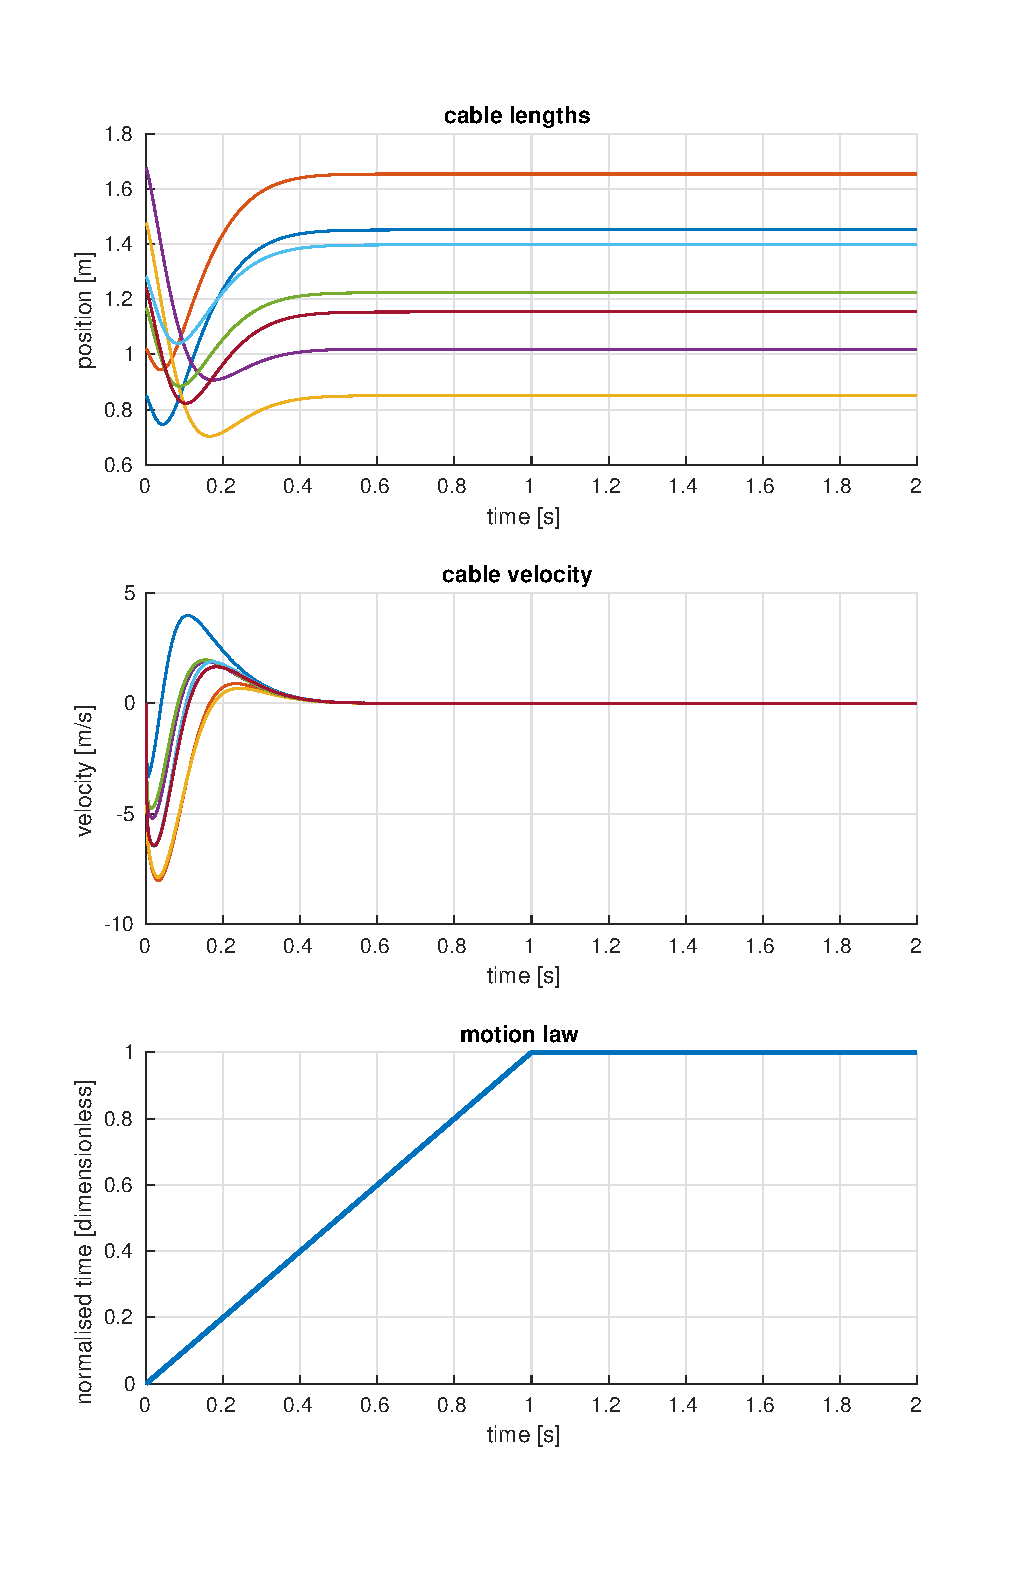
\includegraphics[width=\textwidth]{motion_law_linear}
		\end{minipage}%
		\begin{minipage}{0.45\textwidth}
			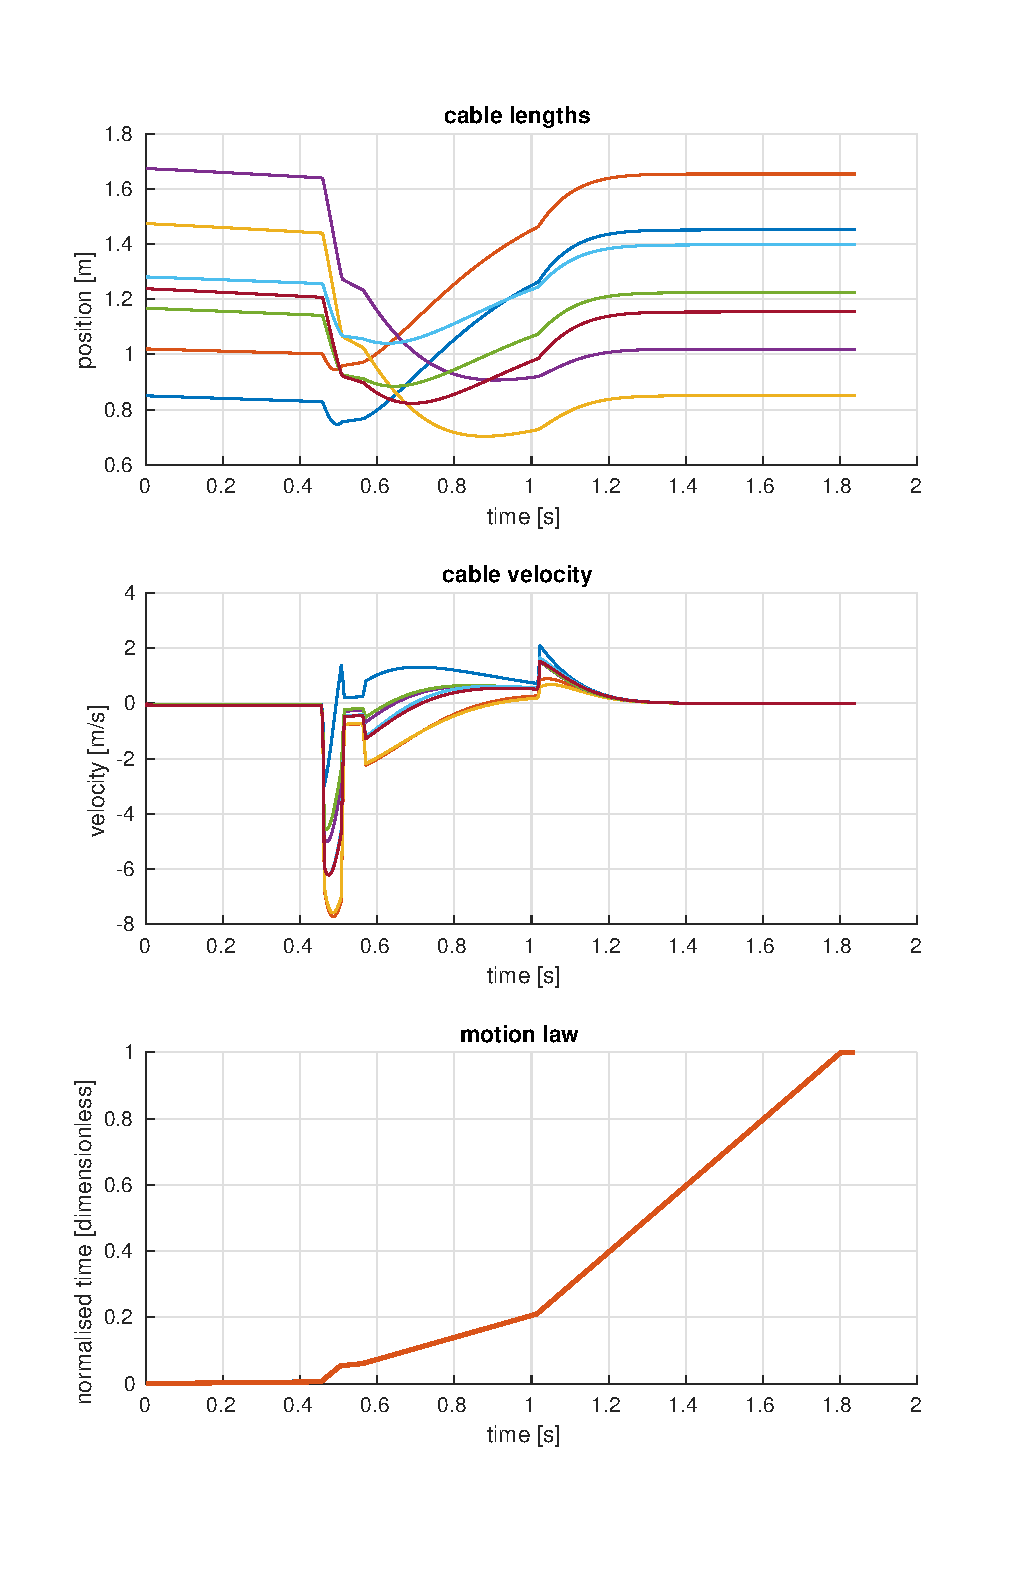
\includegraphics[width=\textwidth]{motion_law_deg_1}
		\end{minipage}
		\caption{No Motion Law (left) and Degree 1 (right) Motion Law}
		\label{fig:motion_law_lin_1}
	\end{figure}

	\begin{figure}[hb]
		\centering
		\begin{minipage}{0.45\textwidth}
			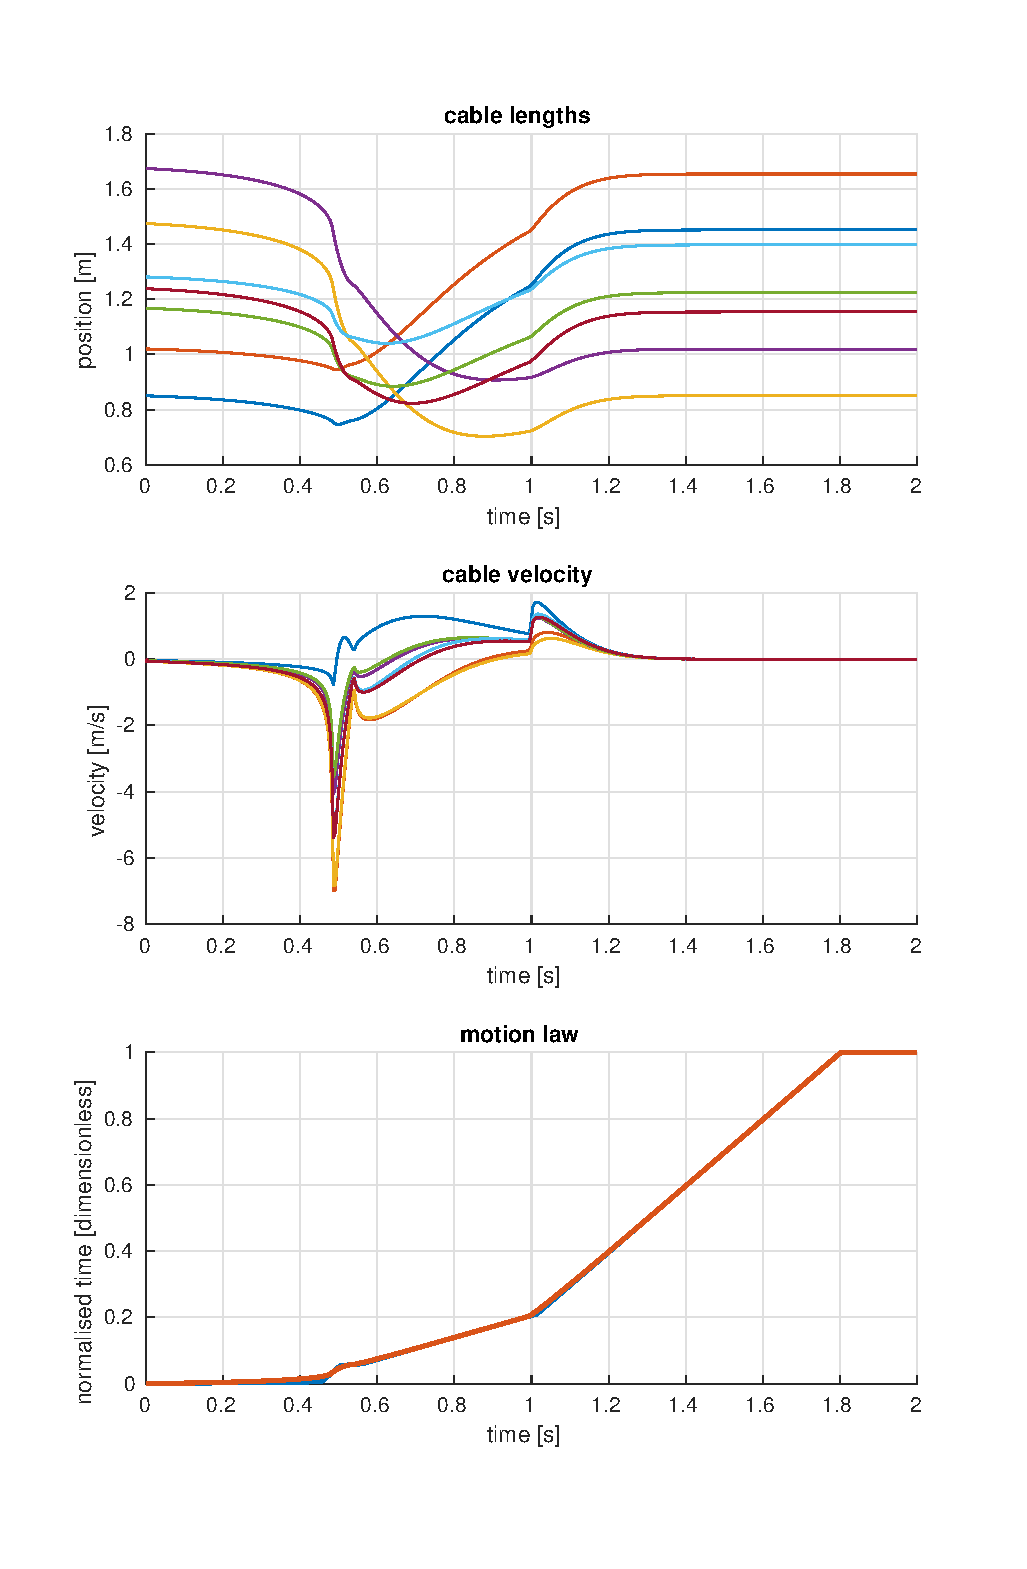
\includegraphics[width=\textwidth]{motion_law_deg_2}
		\end{minipage}%
		\begin{minipage}{0.45\textwidth}
			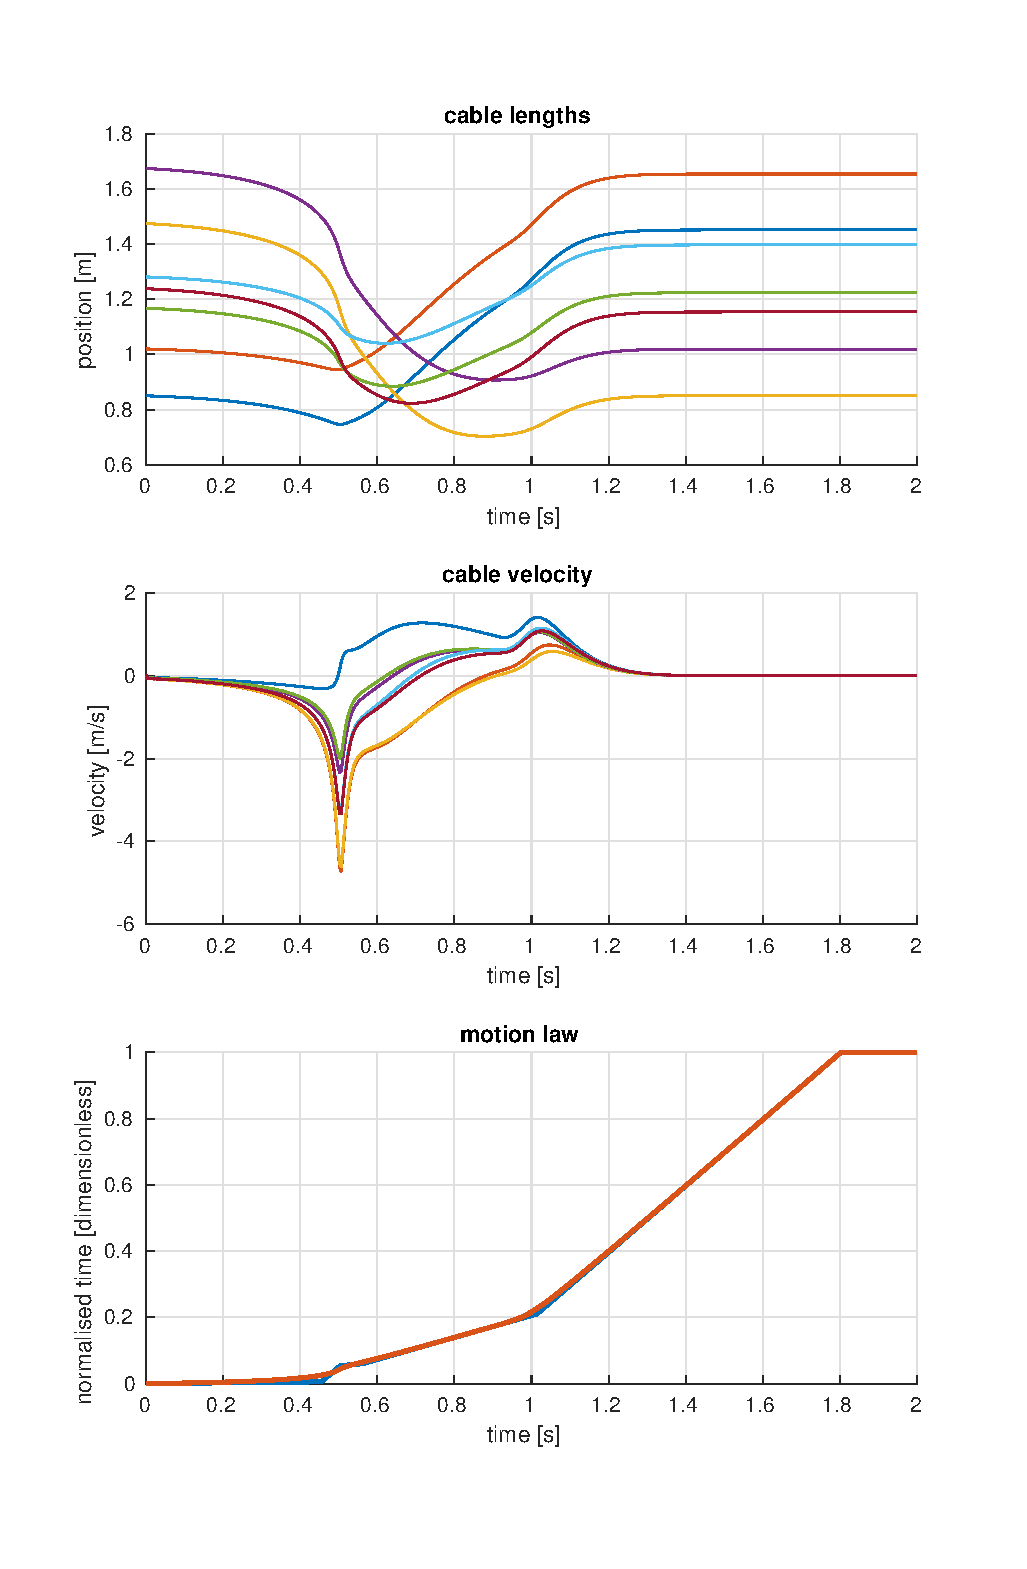
\includegraphics[width=\textwidth]{motion_law_deg_3}
		\end{minipage}%
		\caption{Degree 2 (left) and Degree 3 (right) Motion Law}
		\label{fig:motion_law_2_3}
	\end{figure}

	\begin{figure}[hb]
		\centering
		\begin{minipage}{0.45\textwidth}
			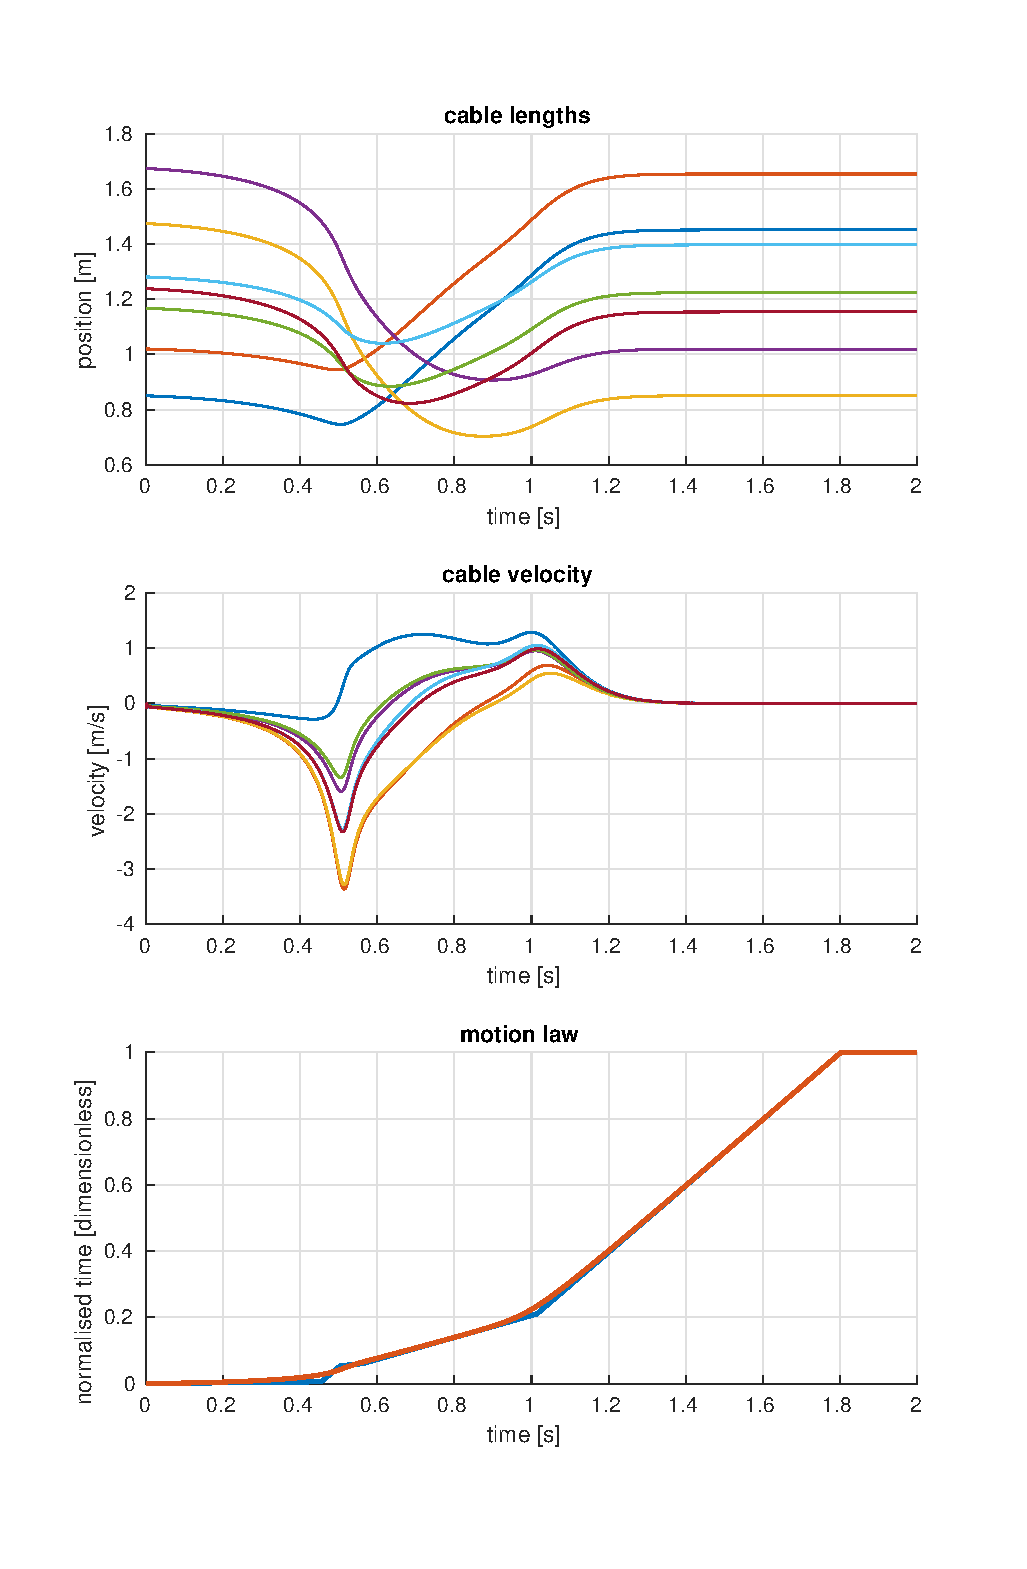
\includegraphics[width=\textwidth]{motion_law_deg_4}
		\end{minipage}%
		\begin{minipage}{0.45\textwidth}
			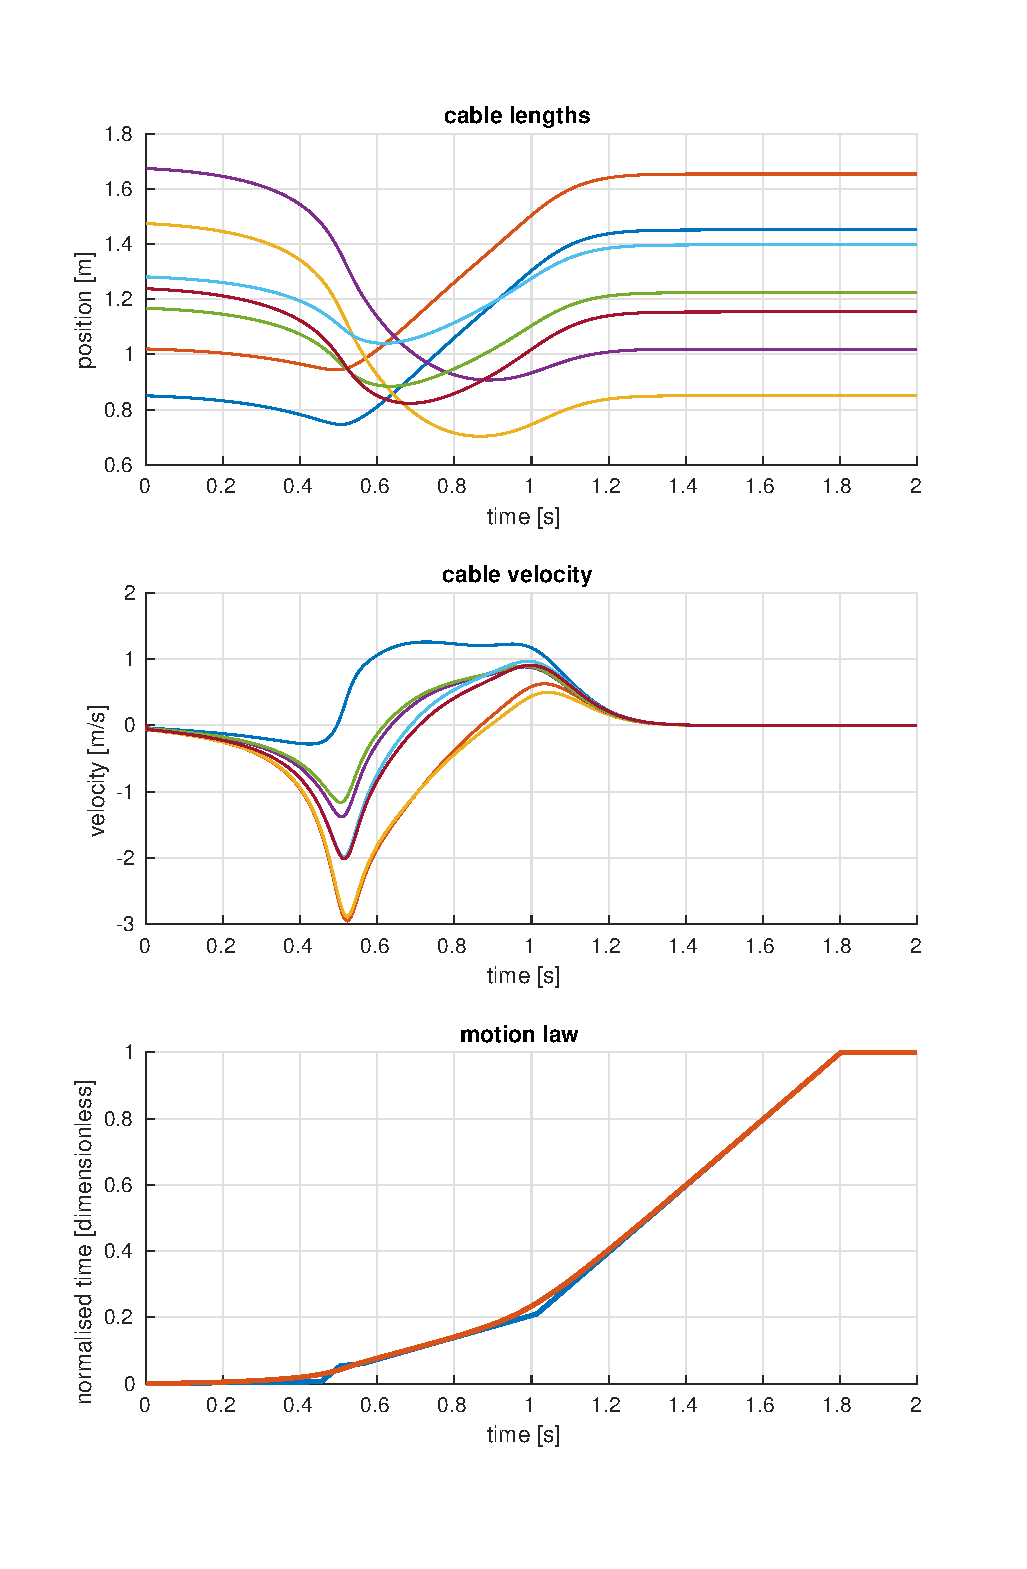
\includegraphics[width=\textwidth]{motion_law_deg_5}
		\end{minipage}%
		\caption{Degree 4 (left) and Degree 5 (right) Motion Law}
		\label{fig:motion_law_4_5}
	\end{figure}

	\begin{figure}[hb]
		\centering
		\begin{minipage}{0.45\textwidth}
			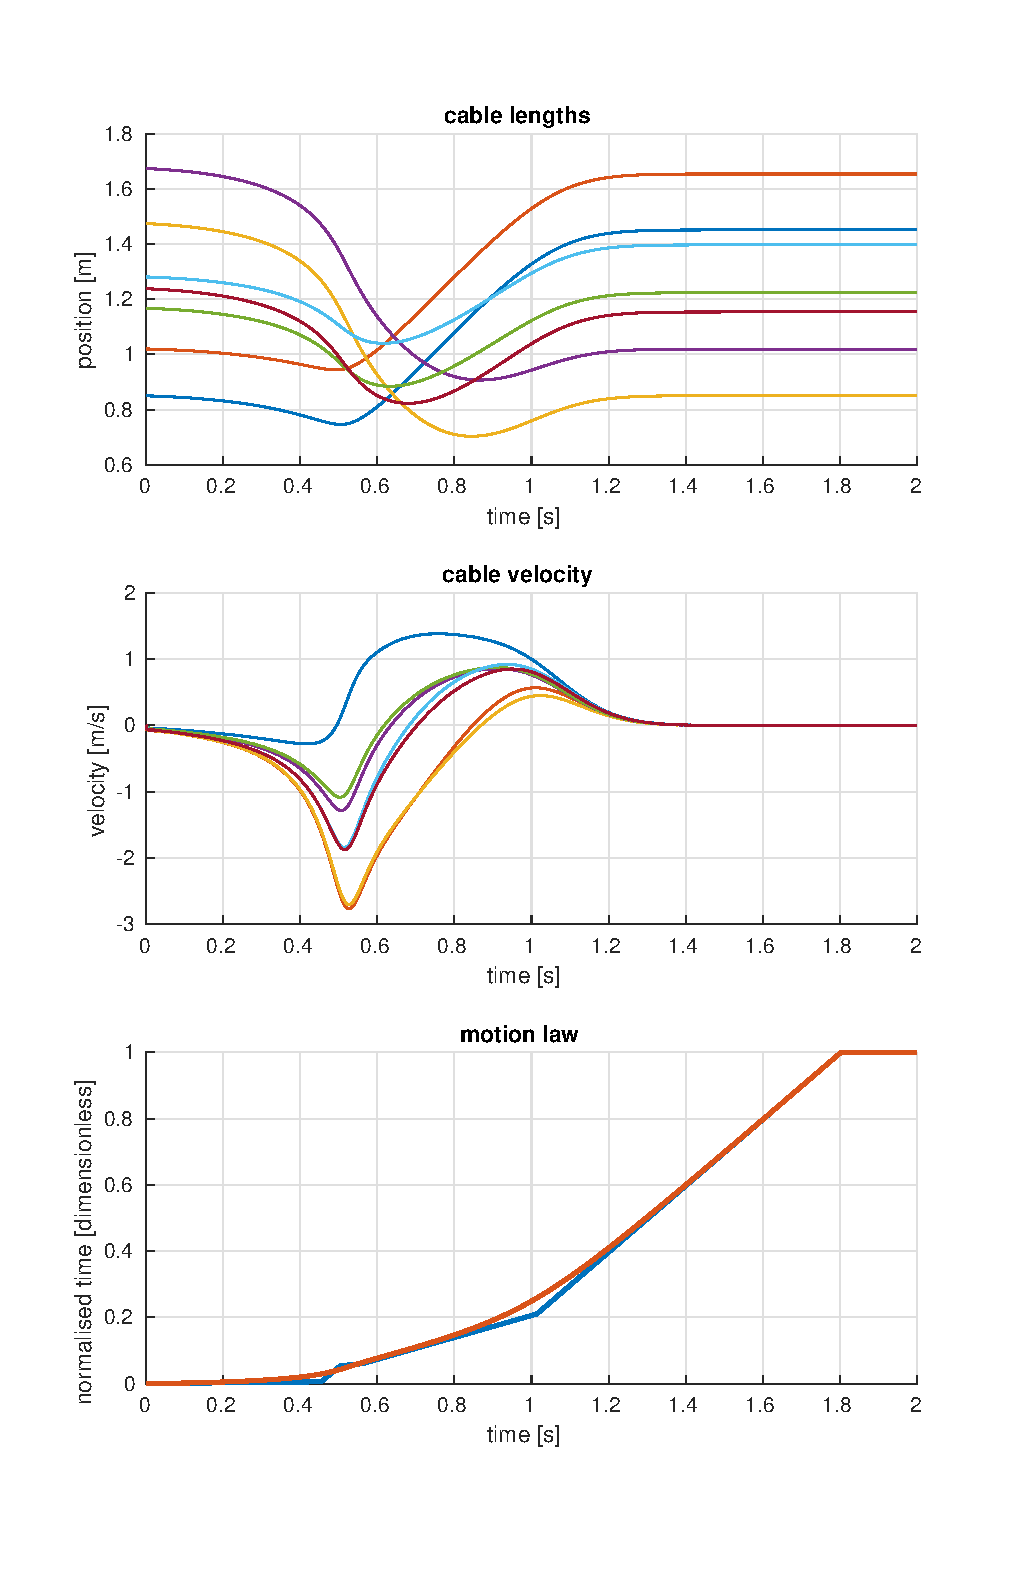
\includegraphics[width=\textwidth]{motion_law_deg_6}
		\end{minipage}%
		\begin{minipage}{0.45\textwidth}
			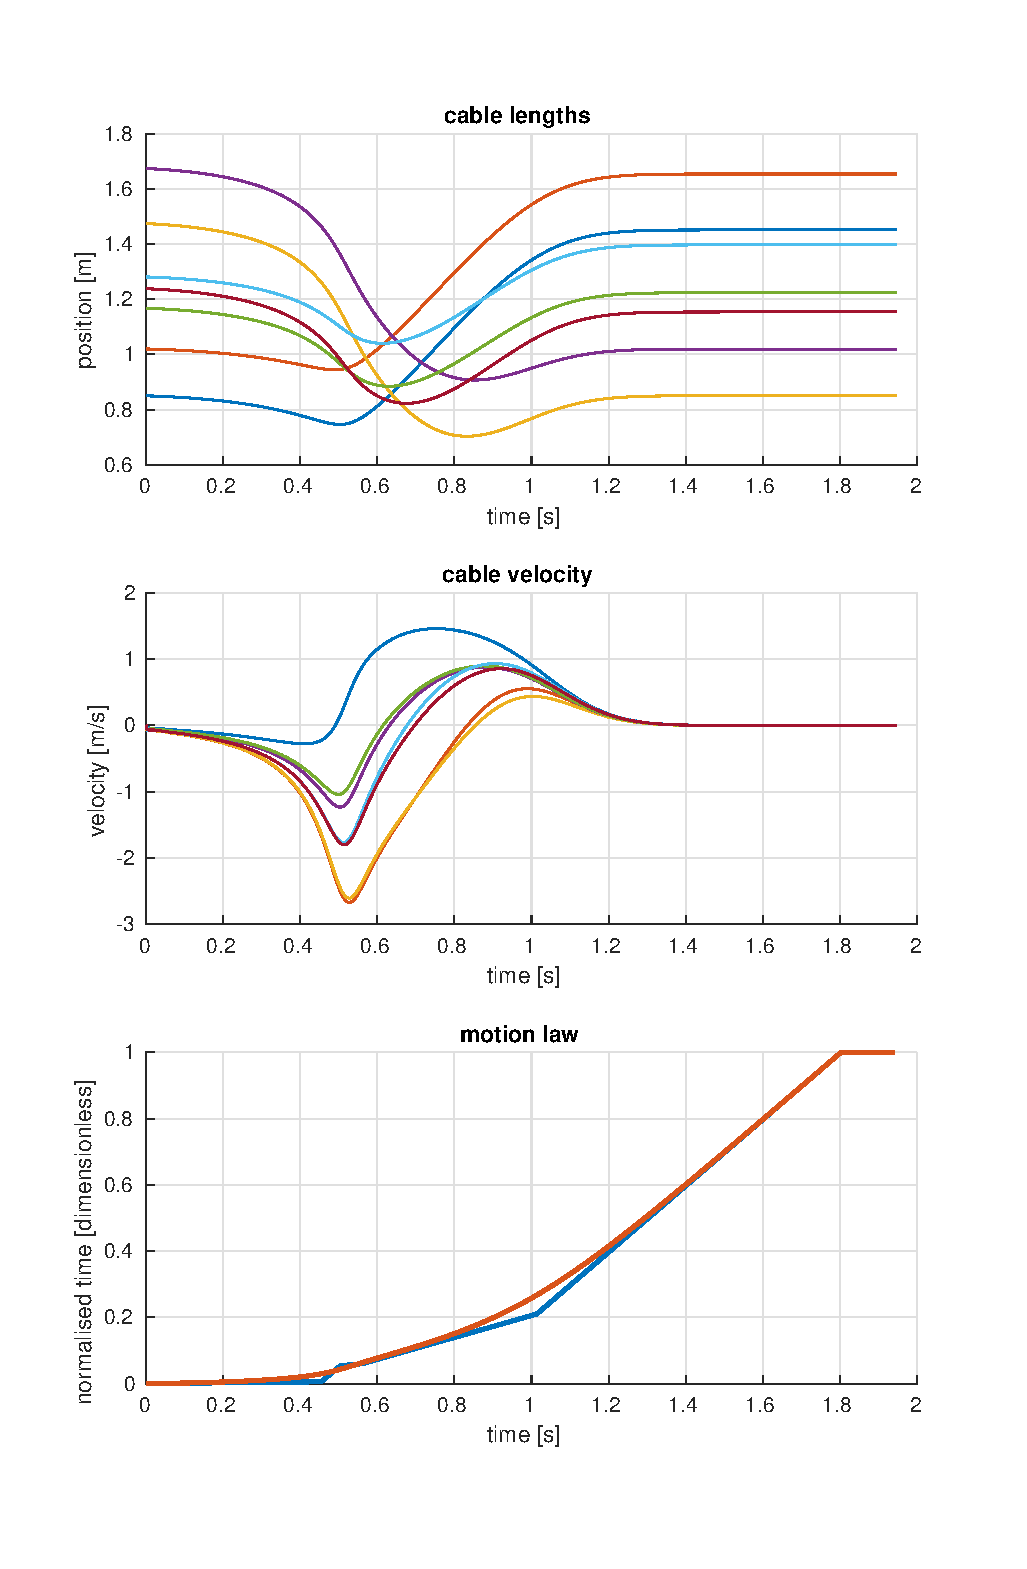
\includegraphics[width=\textwidth]{motion_law_deg_7}
		\end{minipage}%
		\caption{Degree 6 (left) and Degree 7 (right) Motion Law}
		\label{fig:motion_law_6_7}
	\end{figure}

	The left side of Figure~\ref{fig:motion_law_lin_1} shows the case where the
	motion law algorithm is effectively not applied. In this case the motion law
	can be considered to be simply:

	\begin{equation}
		\timenorm =
			\begin{cases}
				\timesym, \quad &0 \leq \timesym \leq 1 \\
				1, \quad &\text{otherwise}
			\end{cases}
	\end{equation}

	Note that the trajectory position and velocity profiles are smooth. This is
	a direct consequence of the B-spline trajectories used. The remaining
	figures show the effect of imposing cable velocity of
	$3\si{\meter\per\second}$ and increasing the degree of the motion law
	spline.

	As can be seen from the figures, a motion law of degree less than 4
	tends to have difficulties starting the trajectory smoothly. This can be
	seen by the cable velocities that exceed the limit of
	$3\si{\meter\per\second}$ initially. This is due to the fact that these
	trajectories do not have smooth jerk profiles.

	Note also how there are jump discontinuities in velocity for a motion law of
	degree 1. These discontinuities occur where the motion law changes slope.
	For a motion law spline of degree 2 (Figure~\ref{fig:motion_law_2_3}, left)
	the jumps in velocity disappear. Note however that there are still sharp
	corners in the velocity profile. This means that the acceleration profile is
	not continuous, which is expected for a motion law of degree 2.

	Furthermore, note how the smoothness of the velocity profile increases as
	the degree of the motion law is increased. However, arbitrarily increasing
	the degree of the motion law spline is not a good approach. In the figures,
	each spline of degree 1 through 7 has the same control points. With this in
	mind, consider the motion laws of degree 5 (Figure~\ref{fig:motion_law_4_5},
	right) and that of degree 7 (Figure~\ref{fig:motion_law_6_7}, right) at time
	$\timesym = 1$. As can be seen, the value of the 7th degree spline differs
	from its control polygon more than the 5th degree spline does. In general,
	higher degree B-splines will tend to move farther away from inner control
	points. For the point $\timesym = 1$ in this example, this lead to the value
	for $\timenorm$ of the spline being higher than that aimed for by the
	control point. This means that, as the degree of the spline is increased,
	there will be points along the trajectory where the robot is farther along
	its path than intended initially. This could lead to excessive velocities.
	As such, the degree of smoothness needs to be balanced with the tendency to
	generate excessive velocities.

	As a good compromise, this thesis uses motion law splines of degree 4 and
	5. Their degree is high enough to at least guarantee smooth jerk, yet remain
	fairly close to the control points. A sample trajectory for these degrees is
	shown in Figure~\ref{fig:motion_law_4_5}.
